\begin{frame}
	\frametitle{Analyseur Sémantique}
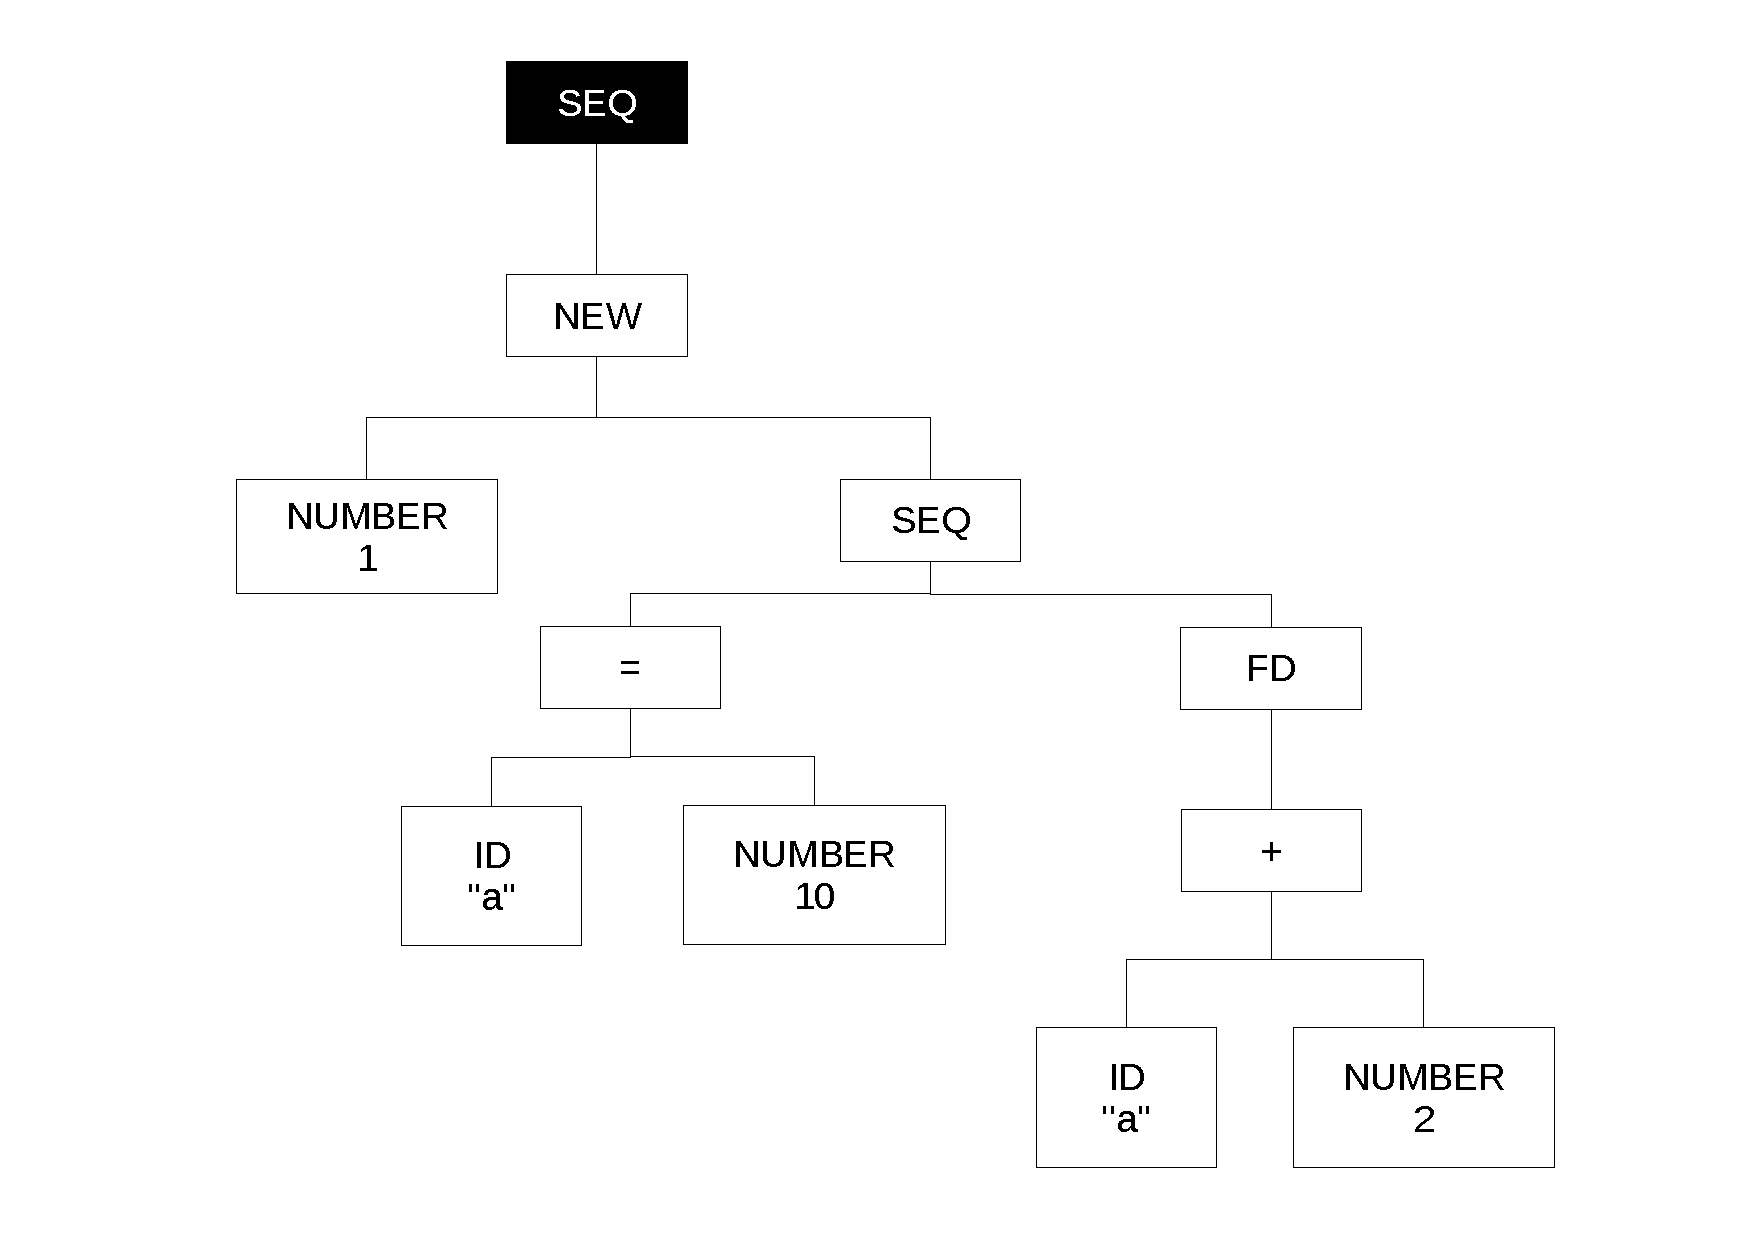
\includegraphics[scale=0.3]{doc/Presentation/img/arbre1.pdf}
\end{frame}

\begin{frame}
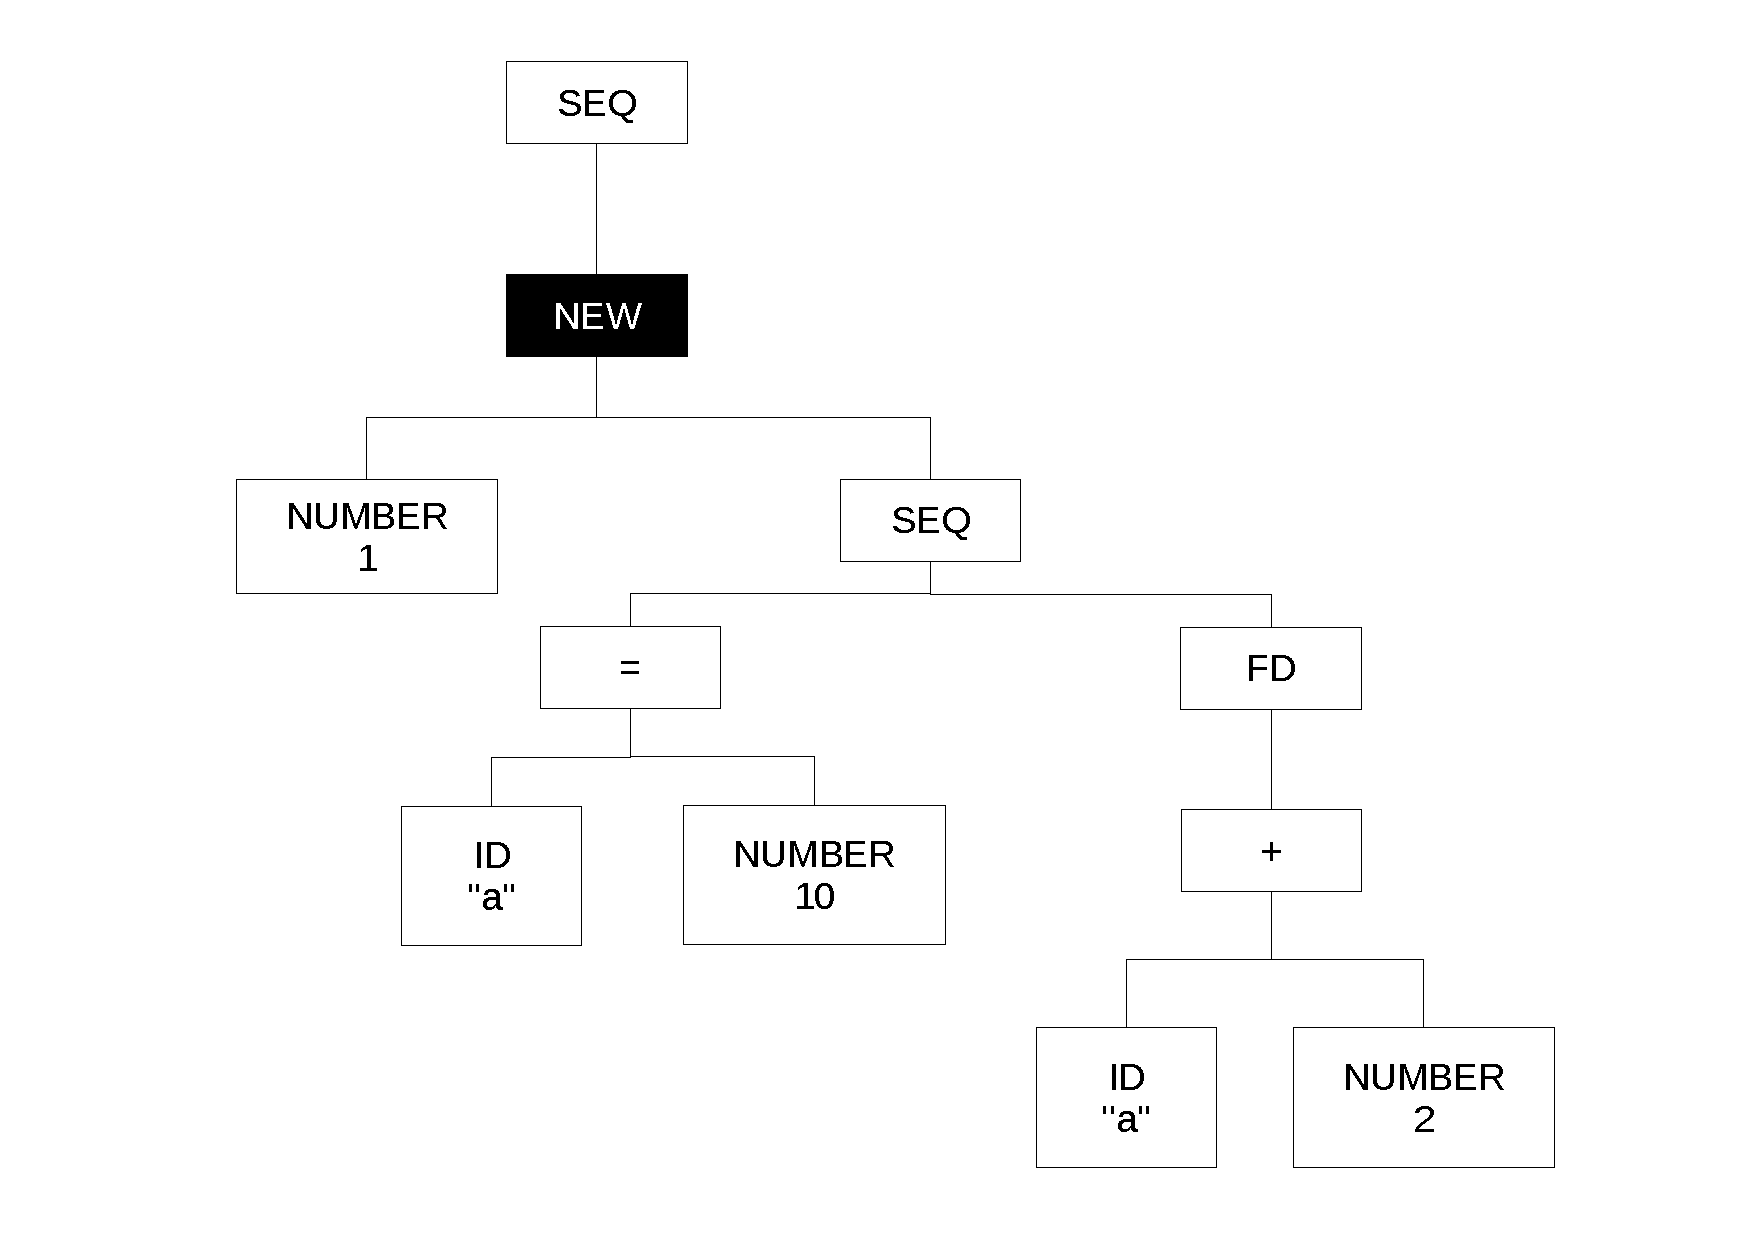
\includegraphics[scale=0.3]{doc/Presentation/img/arbre2.pdf}
\end{frame}

\begin{frame}
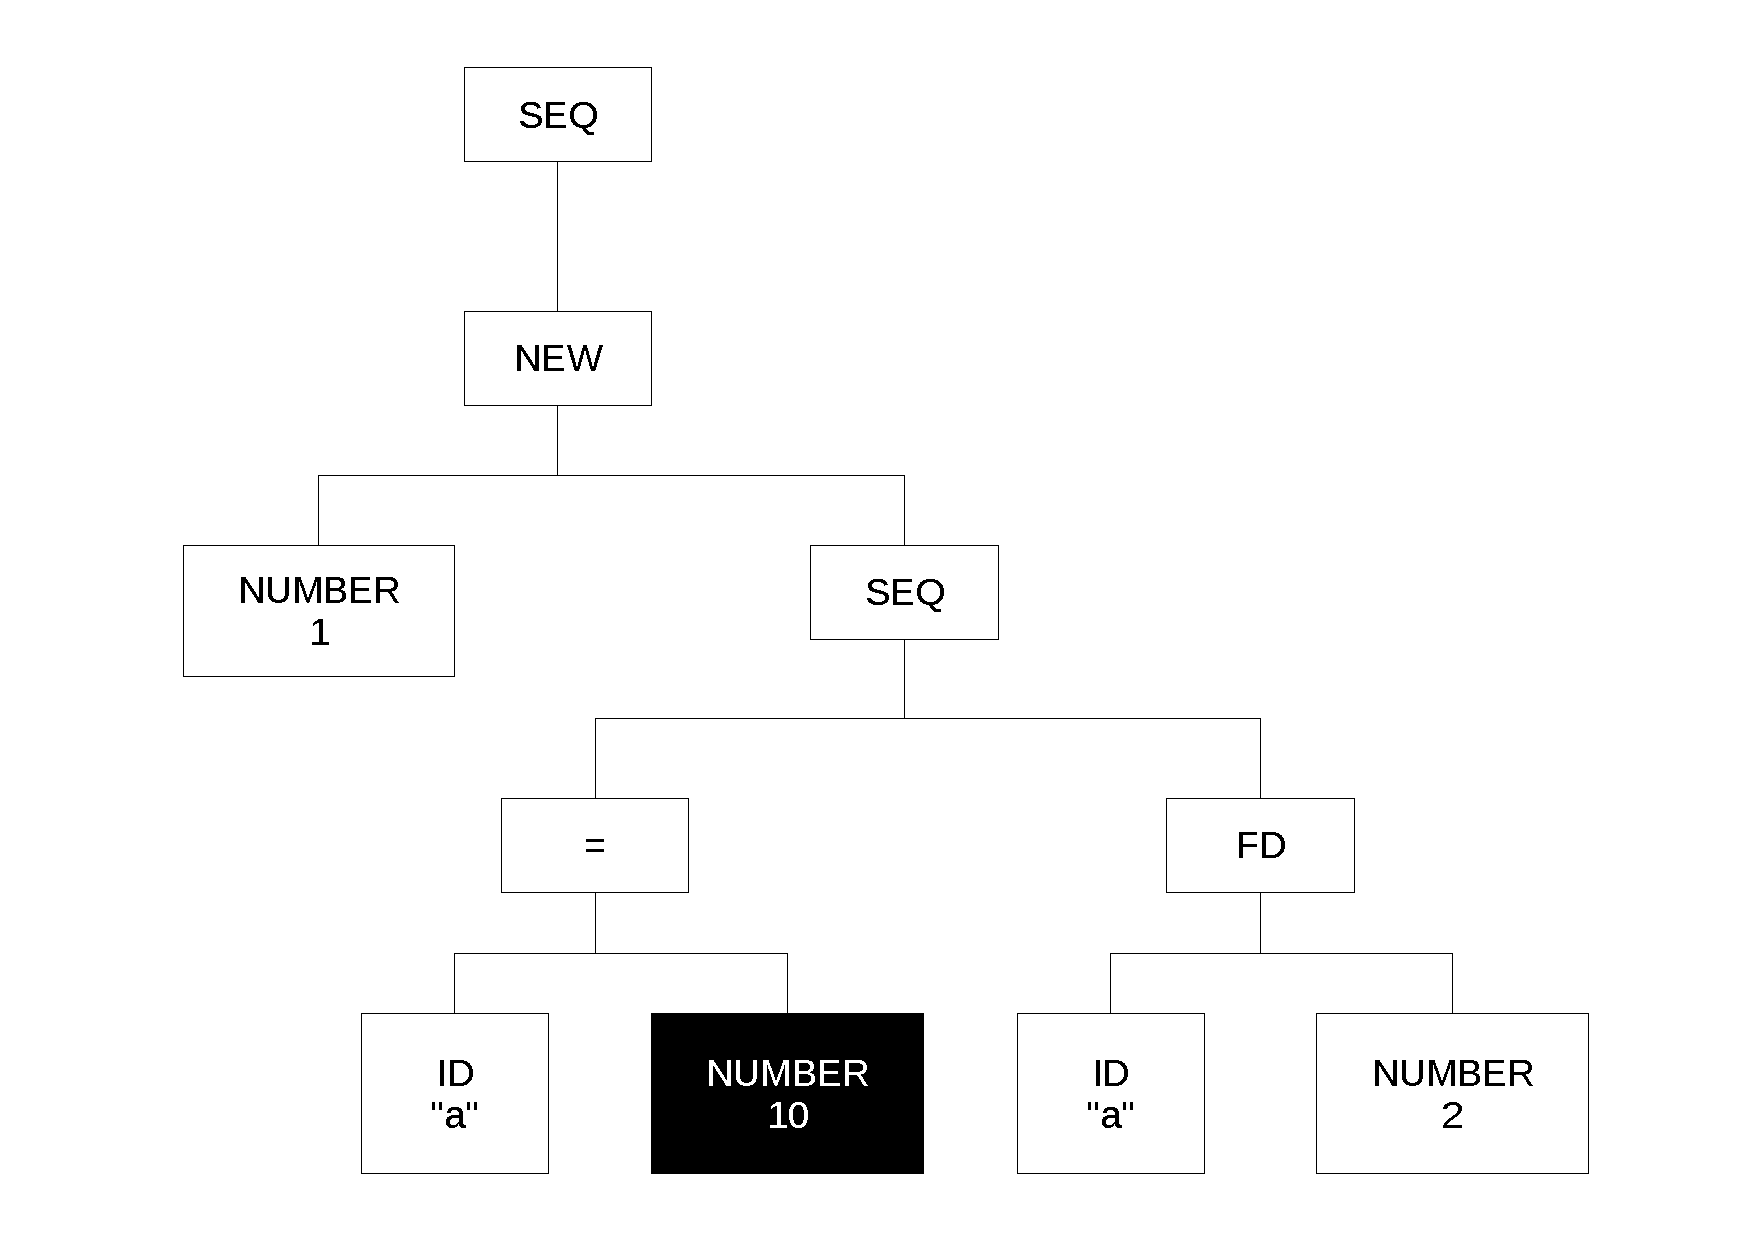
\includegraphics[scale=0.3]{doc/Presentation/img/arbre3.pdf}
\end{frame}

\begin{frame}[fragile]
	\begin{lstlisting}[language=Stibbons]
new agent {
  a = 10
  fd a + 2
}

1 new agent {
  a = 10
  fd a + 2
}
	\end{lstlisting}
\end{frame}

\begin{frame}
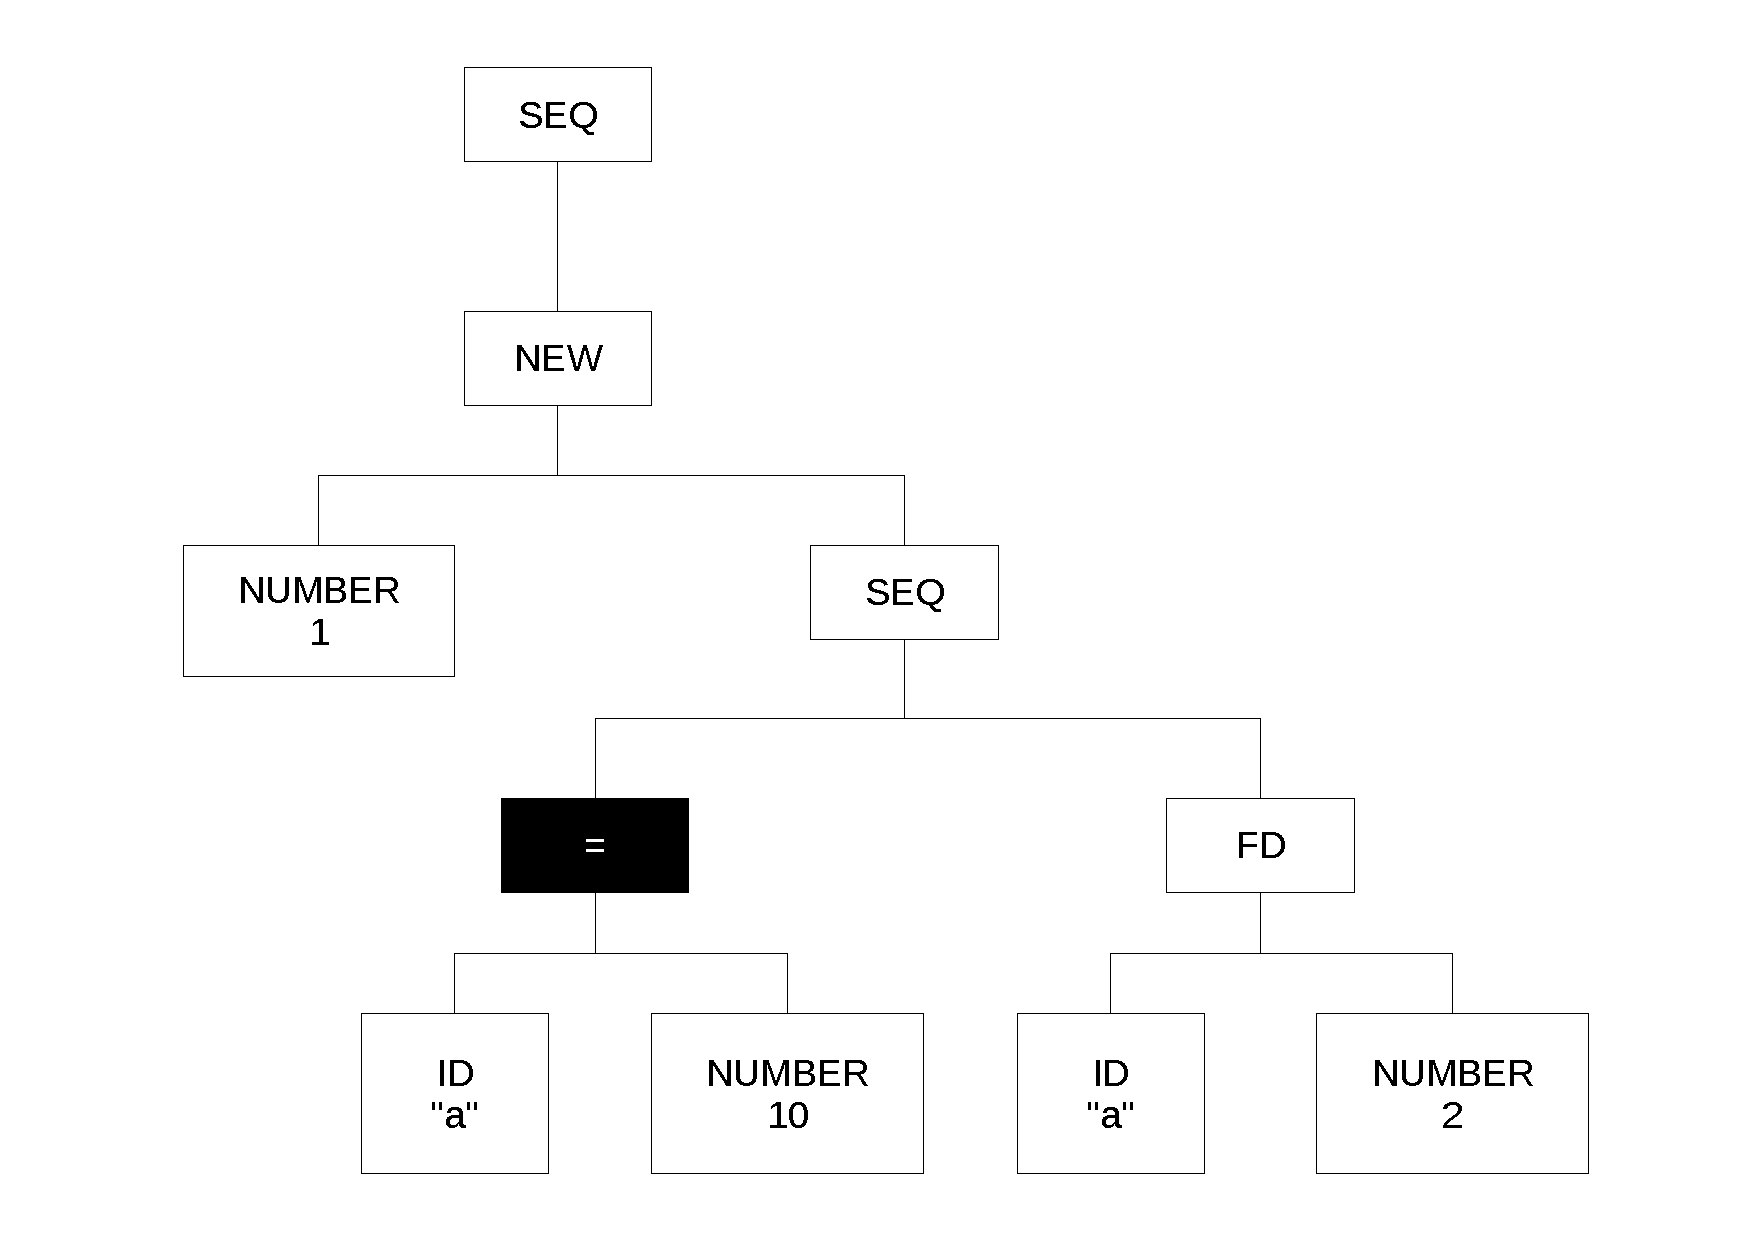
\includegraphics[scale=0.3]{doc/Presentation/img/arbre4.pdf}
\end{frame}

\begin{frame}
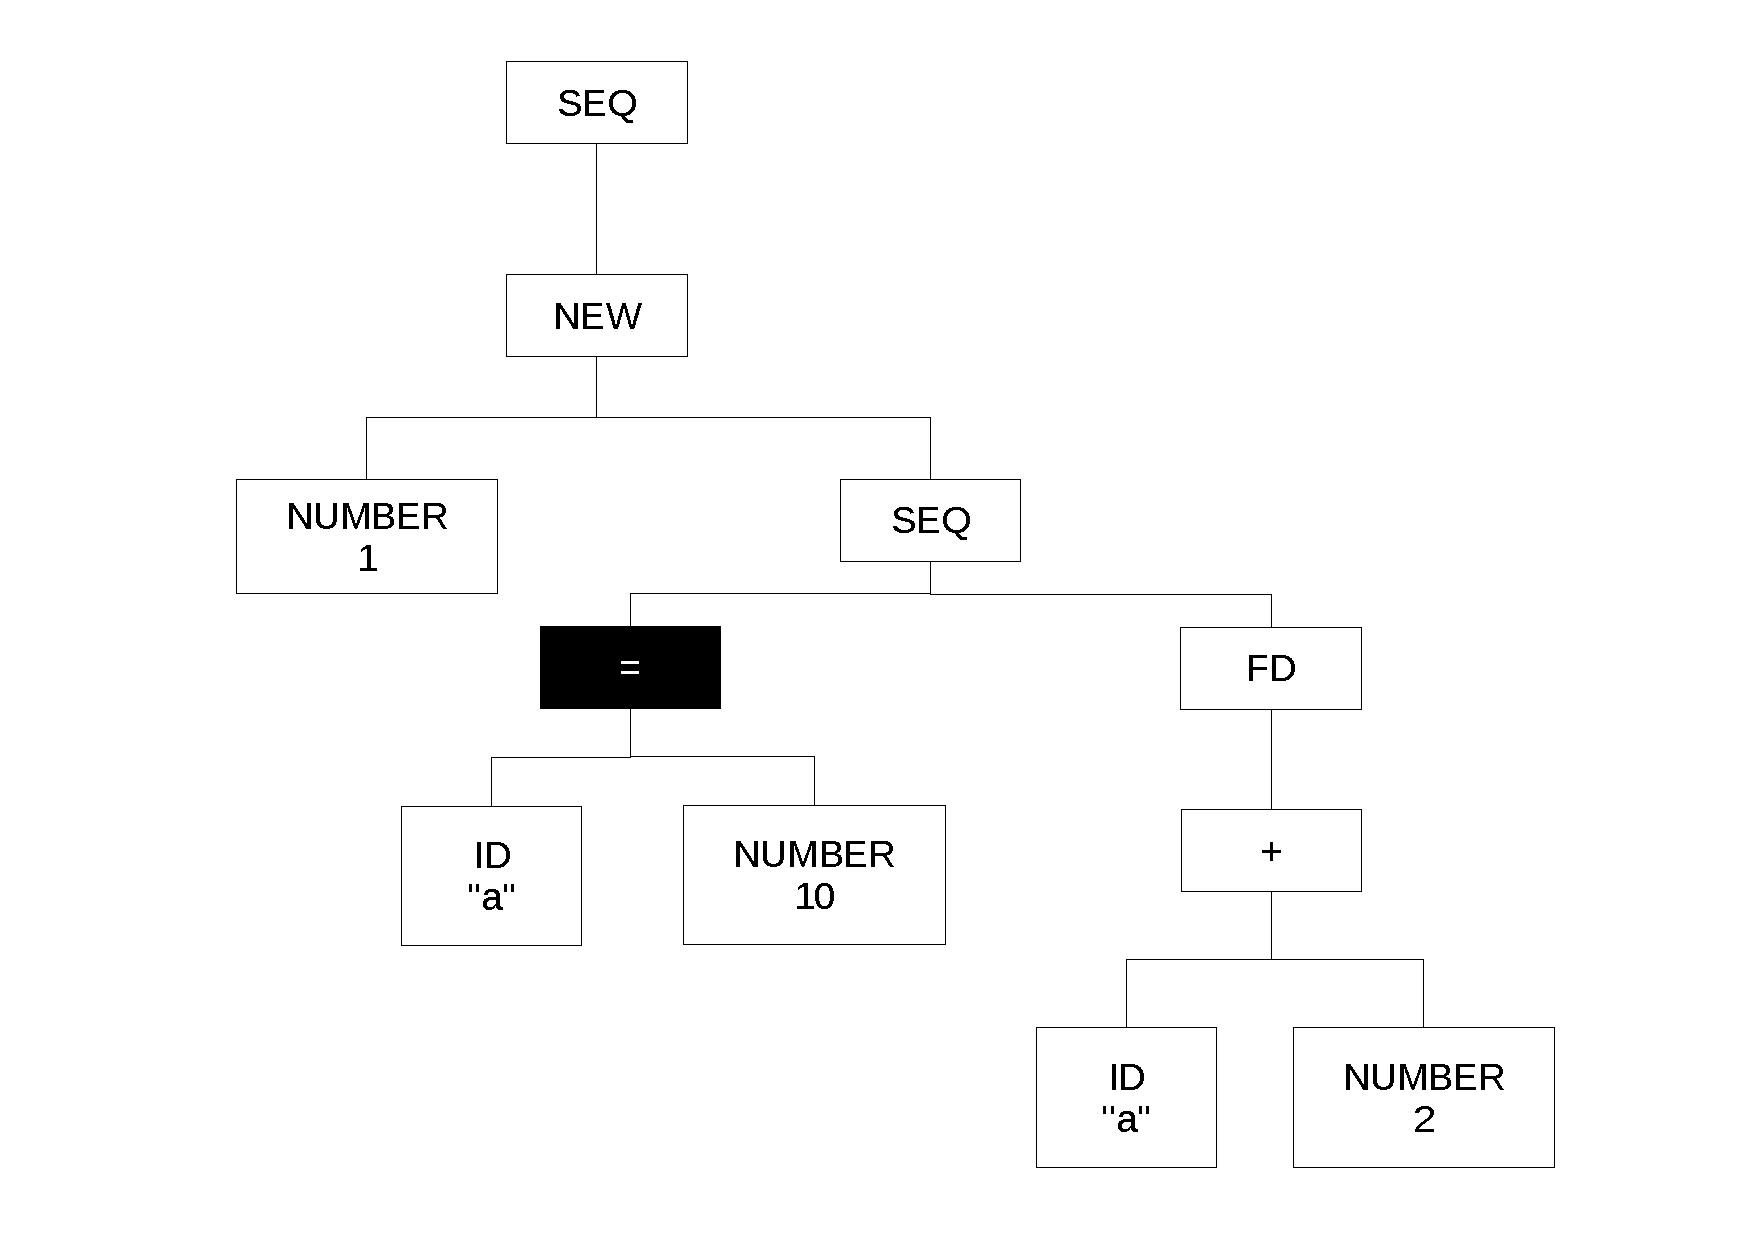
\includegraphics[scale=0.3]{doc/Presentation/img/arbre5.pdf}
\end{frame}

\begin{frame}
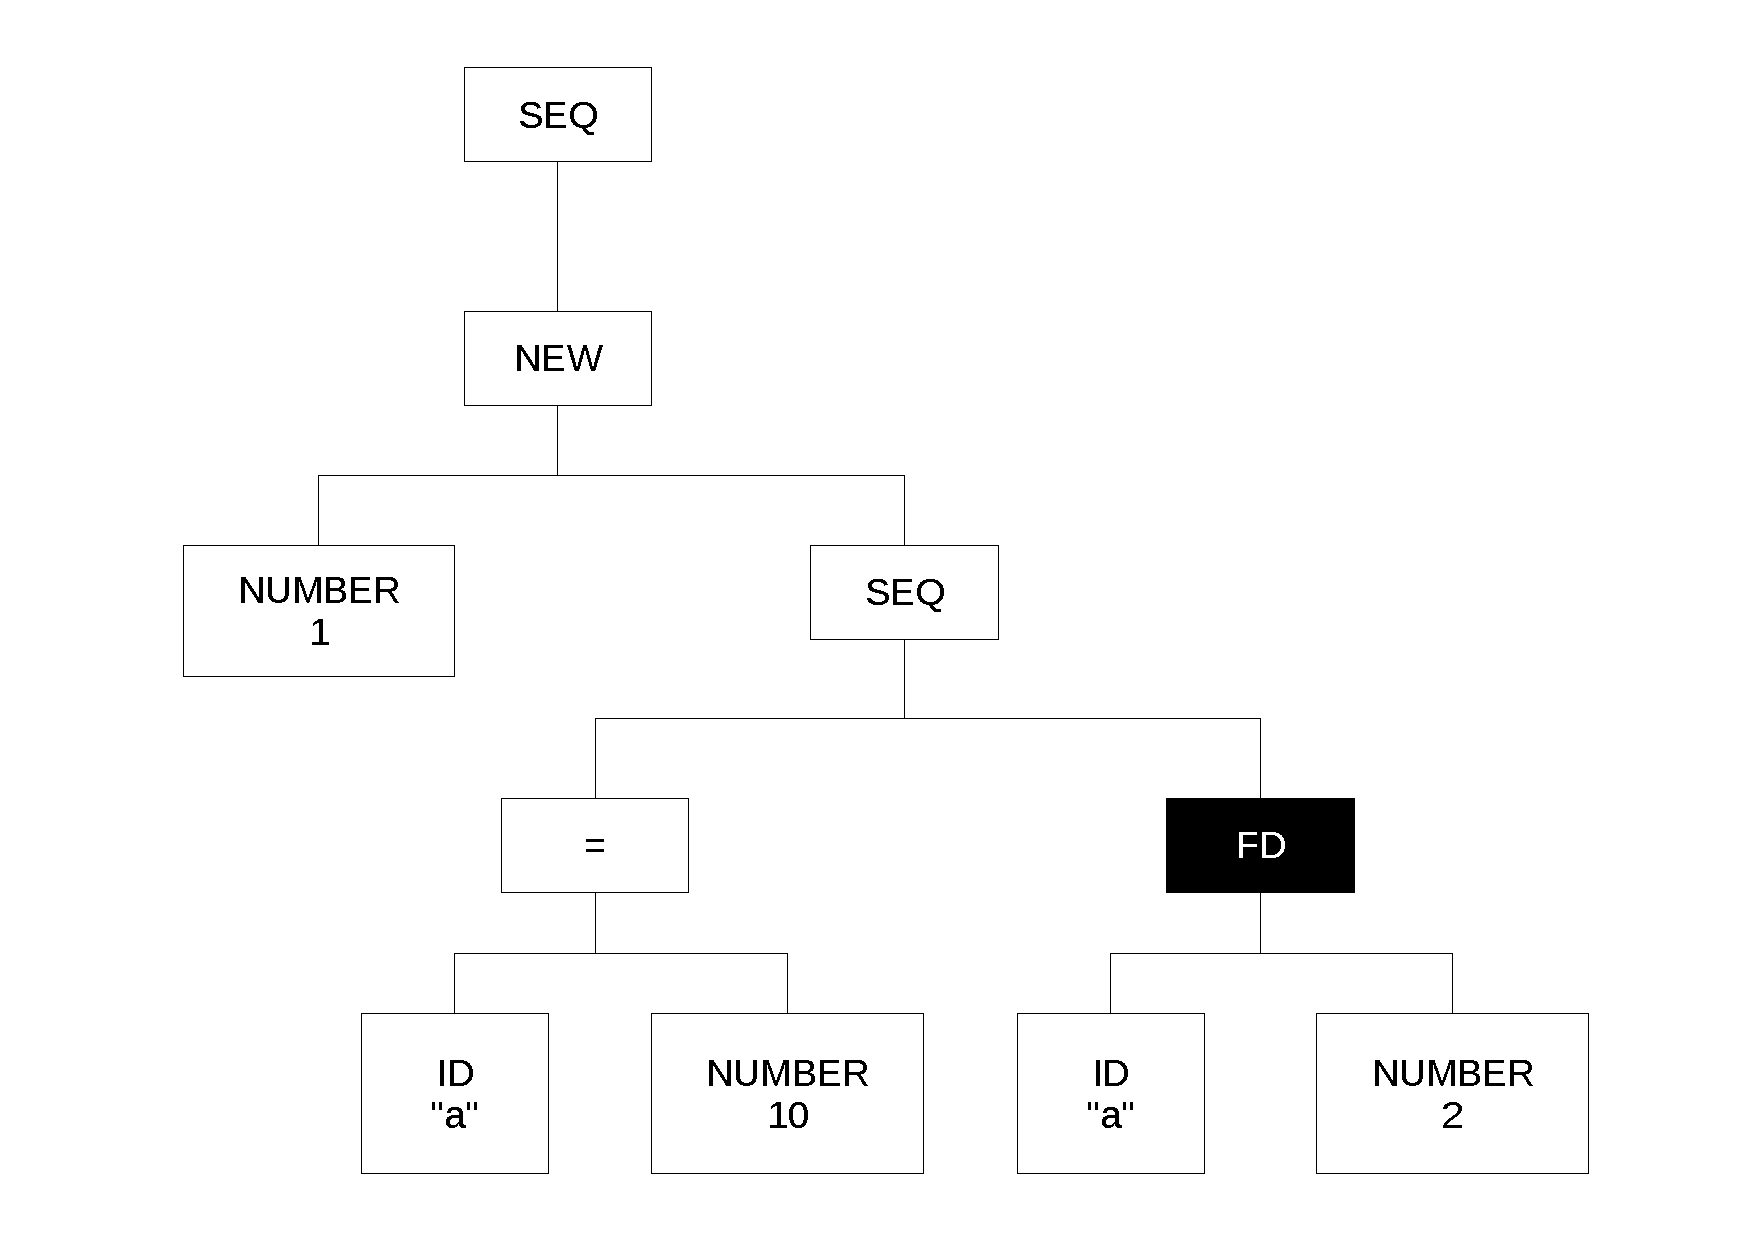
\includegraphics[scale=0.3]{doc/Presentation/img/arbre7.pdf}
\end{frame}

\begin{frame}
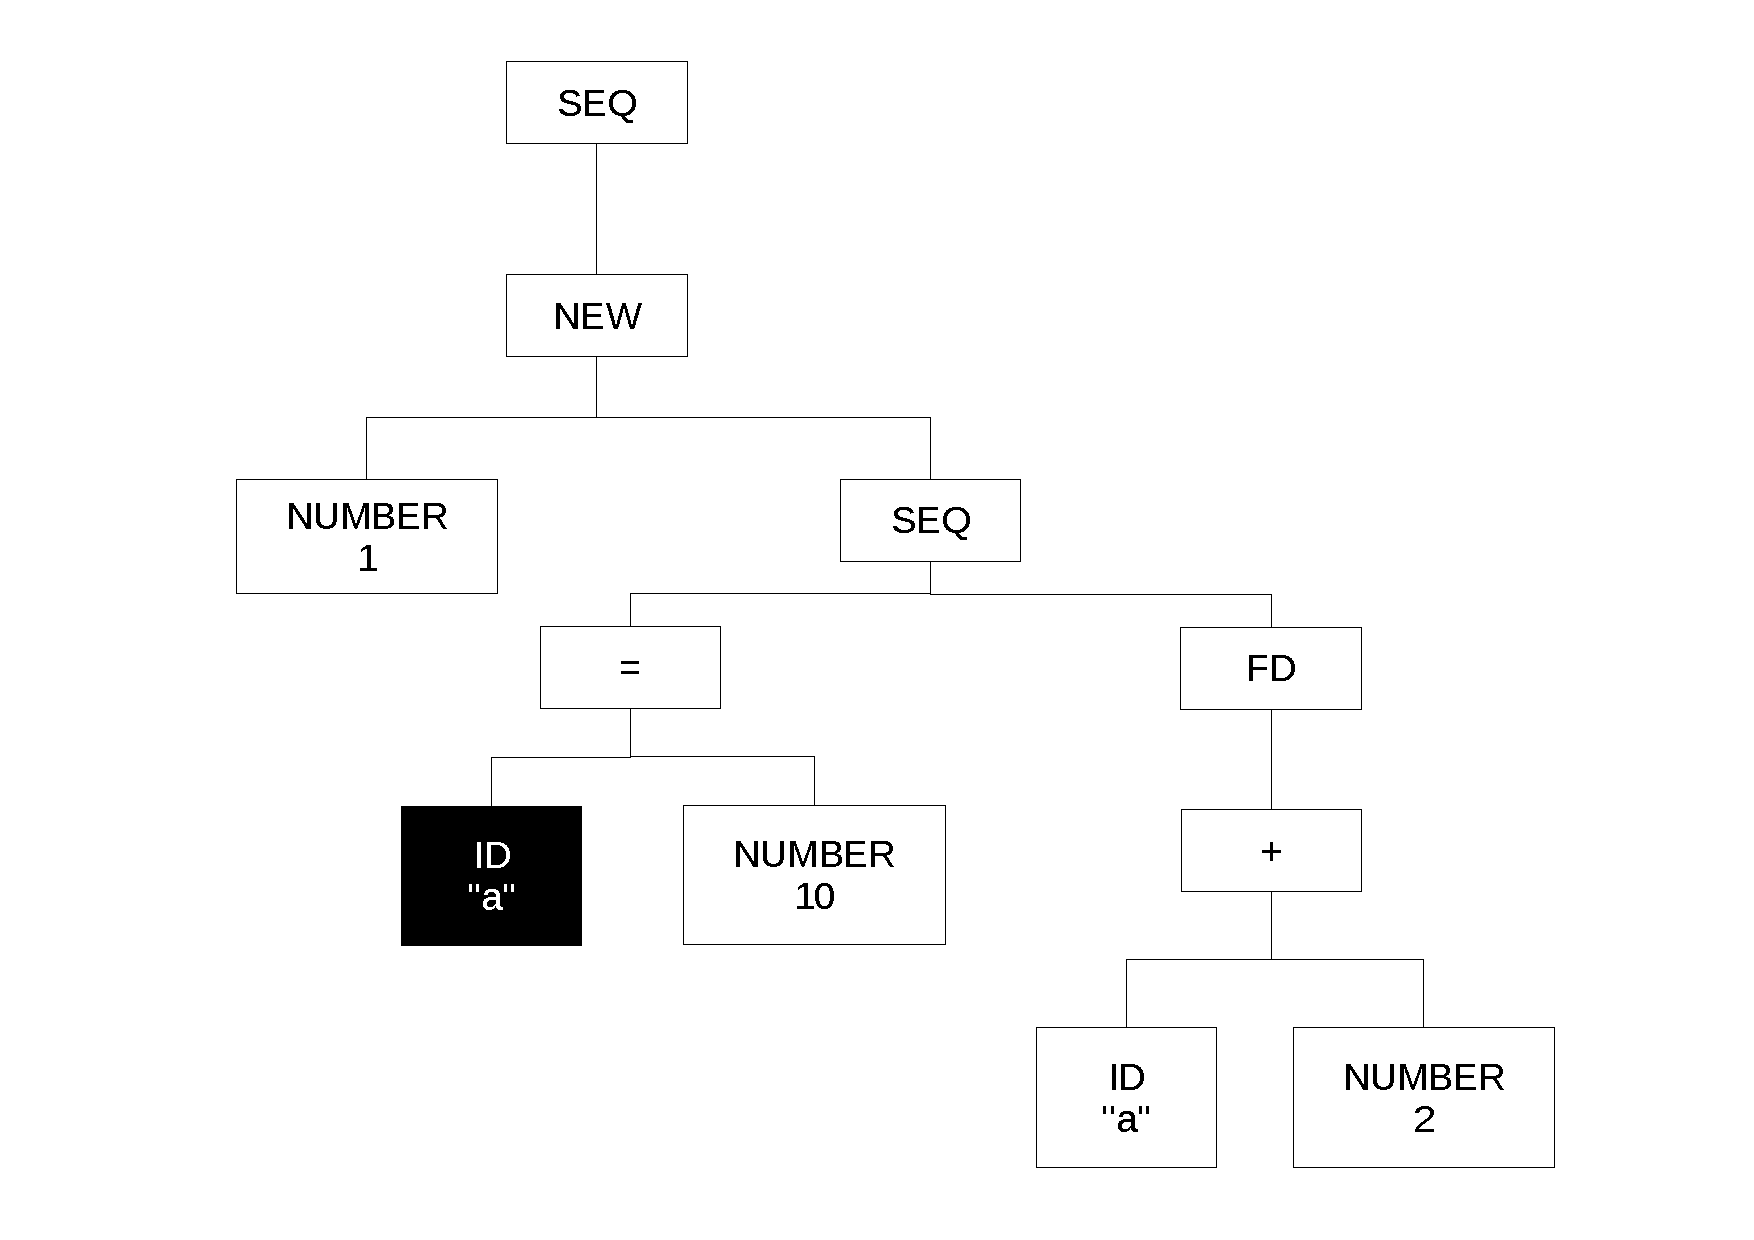
\includegraphics[scale=0.3]{doc/Presentation/img/arbre6.pdf}
\end{frame}

\begin{frame}
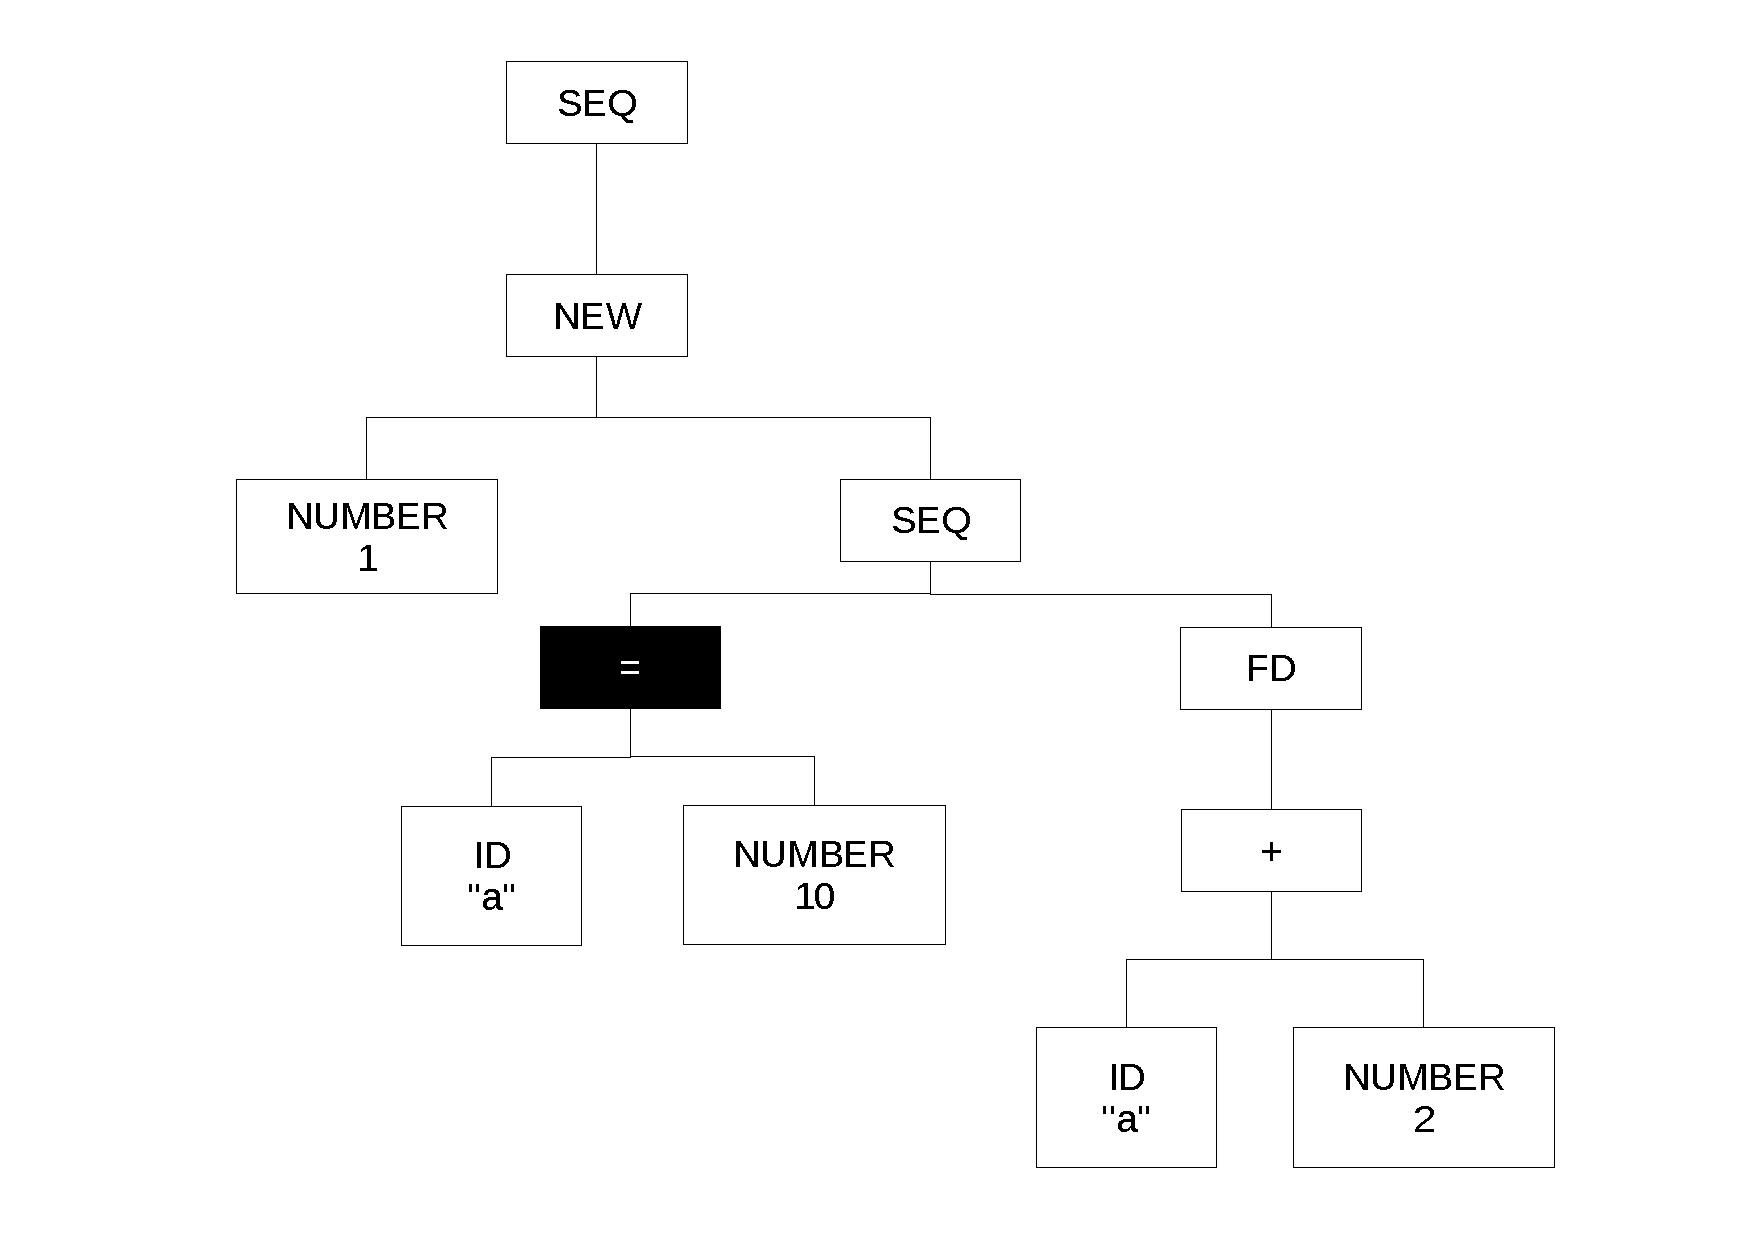
\includegraphics[scale=0.3]{doc/Presentation/img/arbre5.pdf}
\end{frame}

\begin{frame}
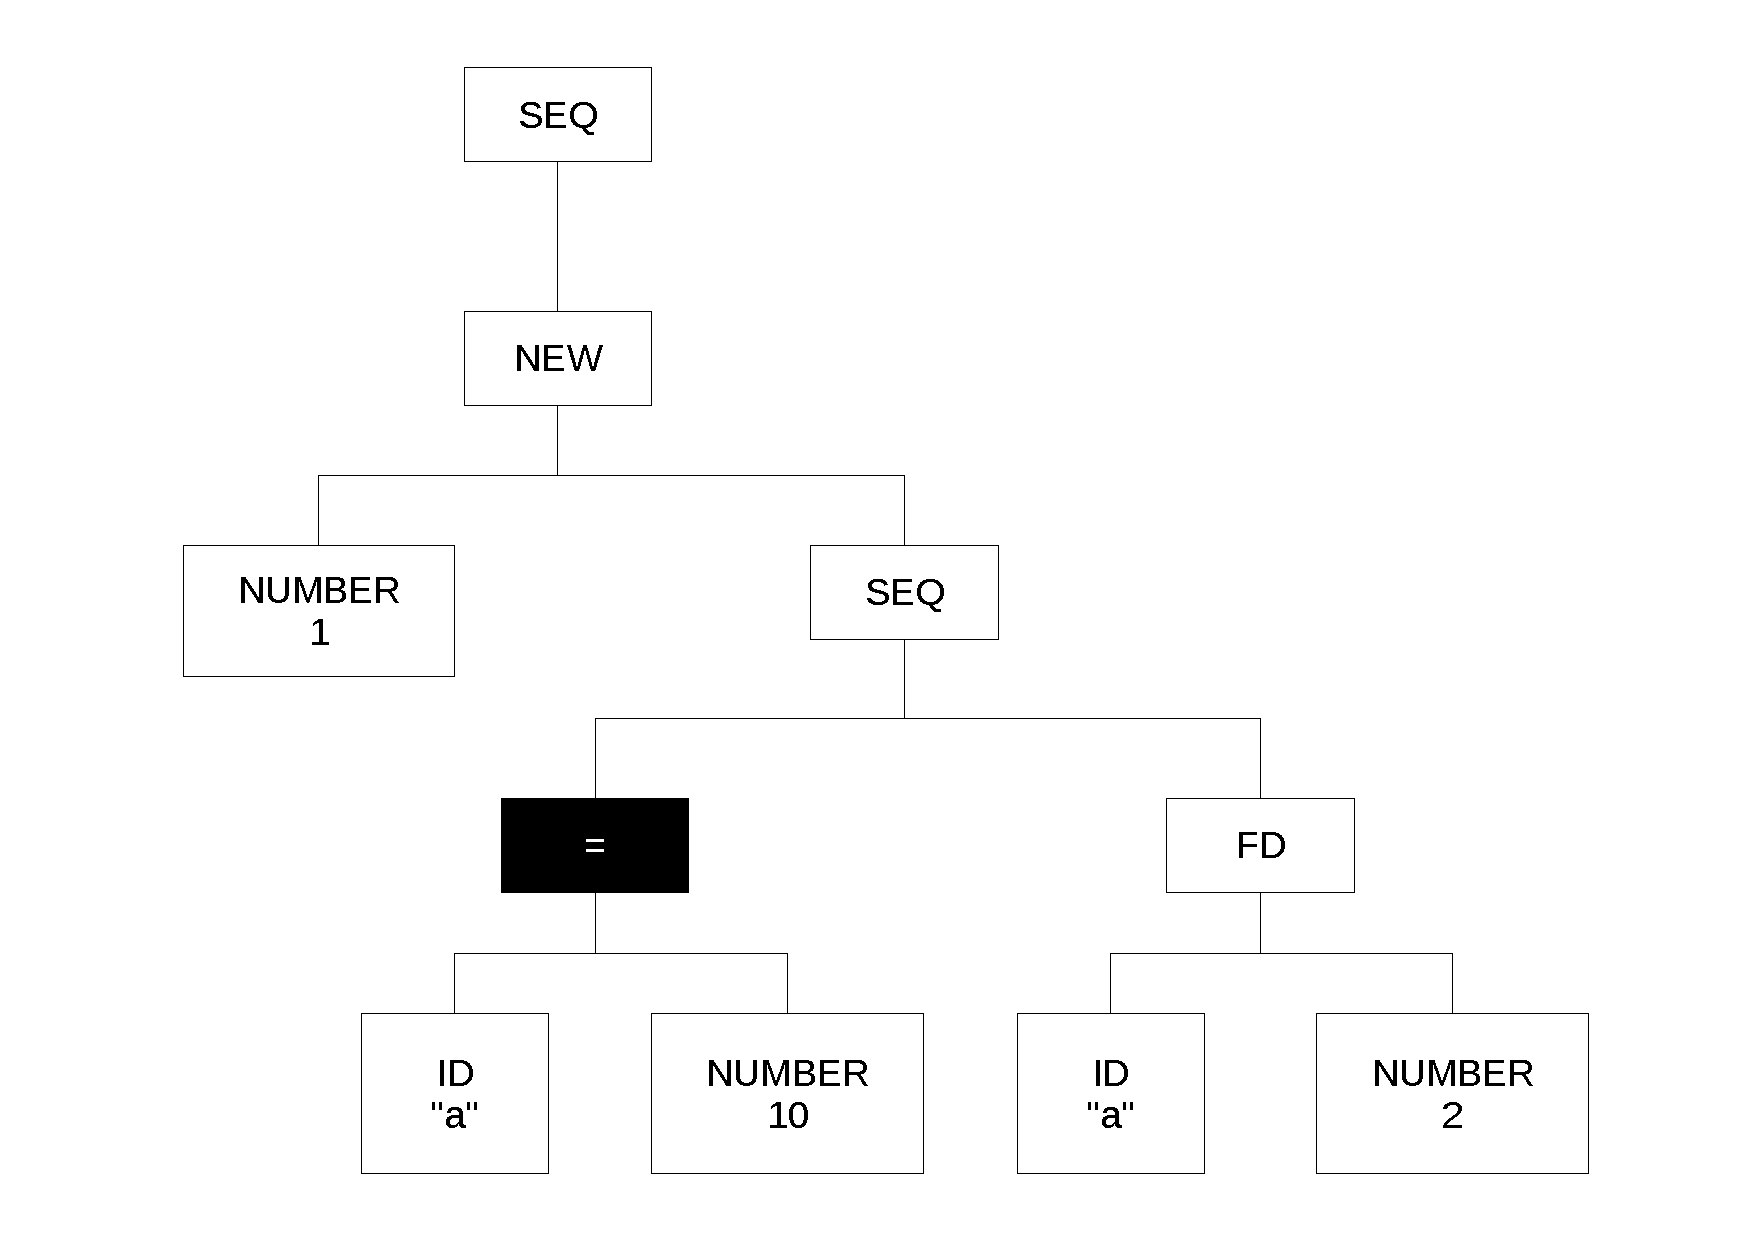
\includegraphics[scale=0.3]{doc/Presentation/img/arbre4.pdf}
\end{frame}

\begin{frame}
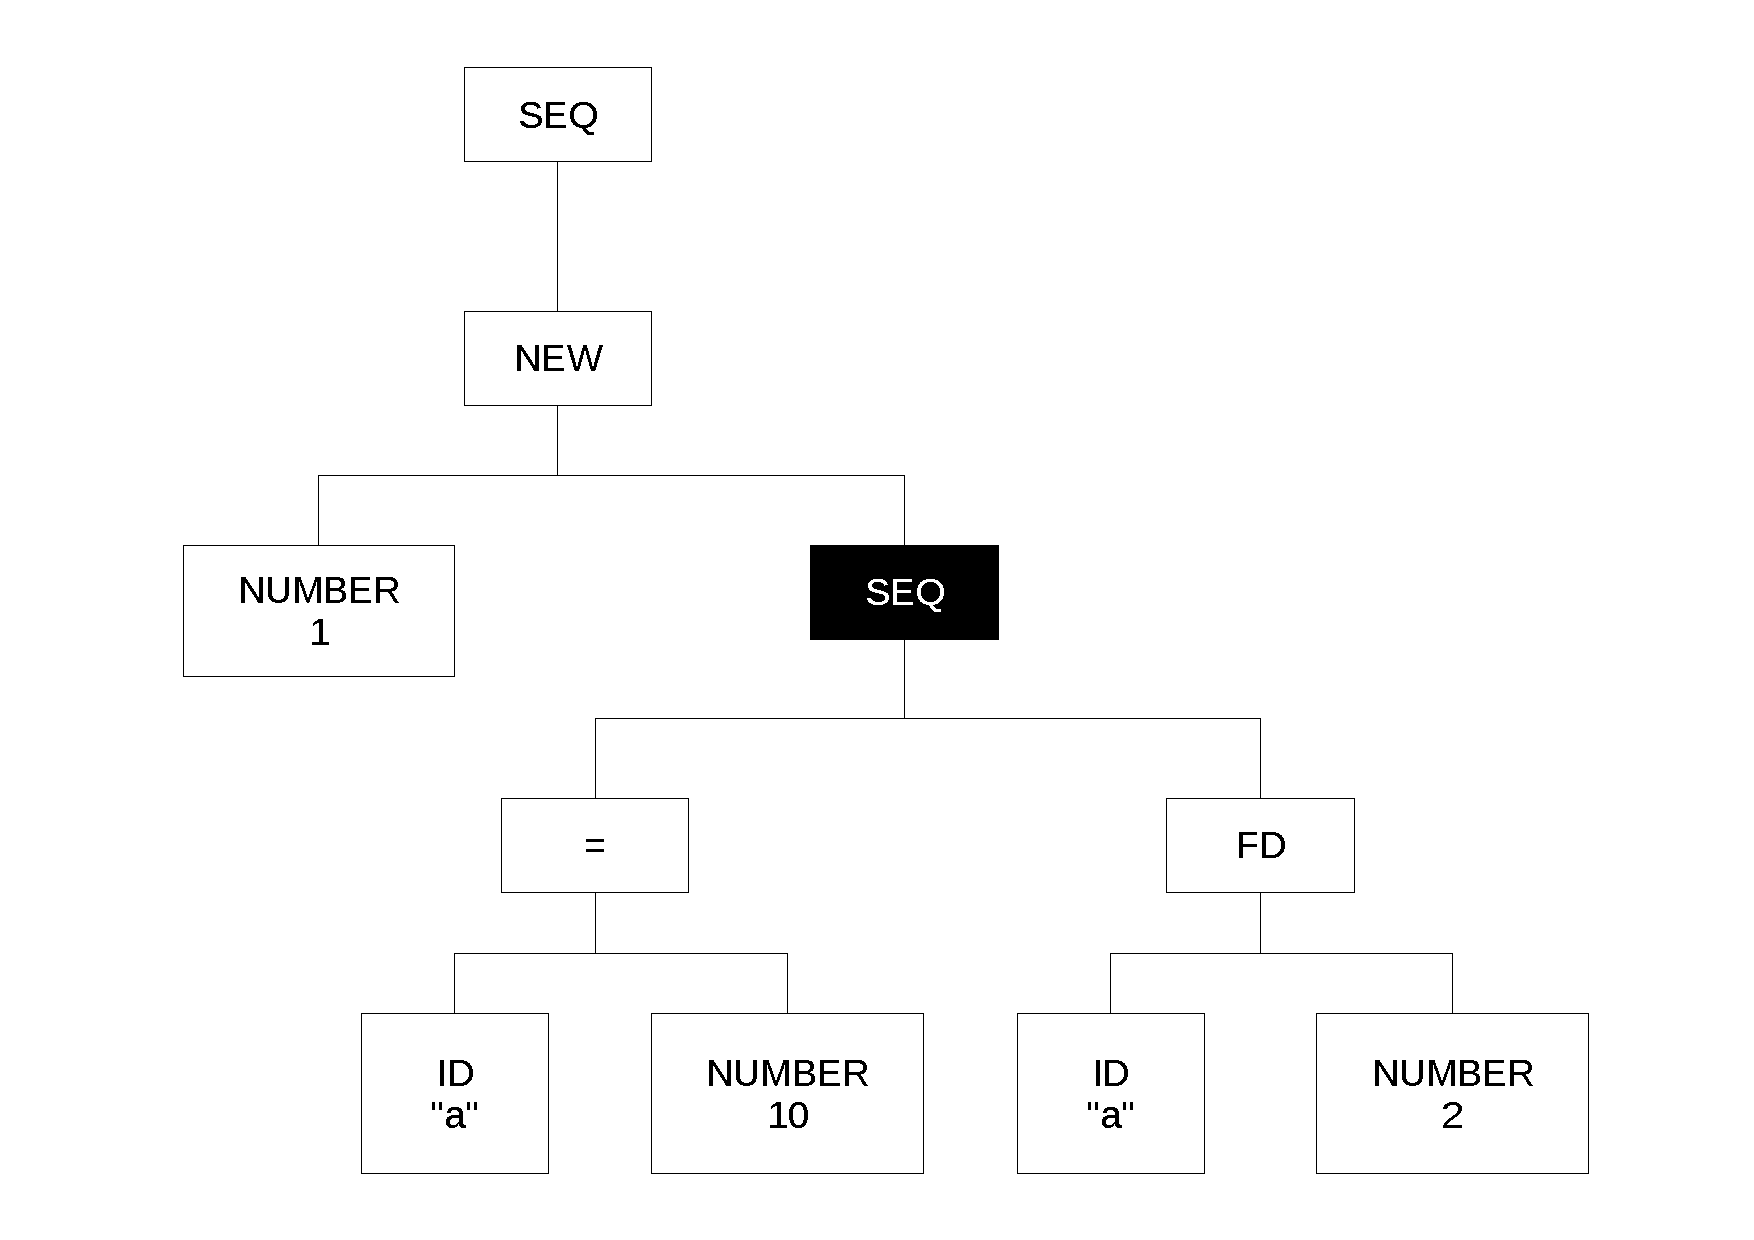
\includegraphics[scale=0.3]{doc/Presentation/img/arbre8.pdf}
\end{frame}

\begin{frame}
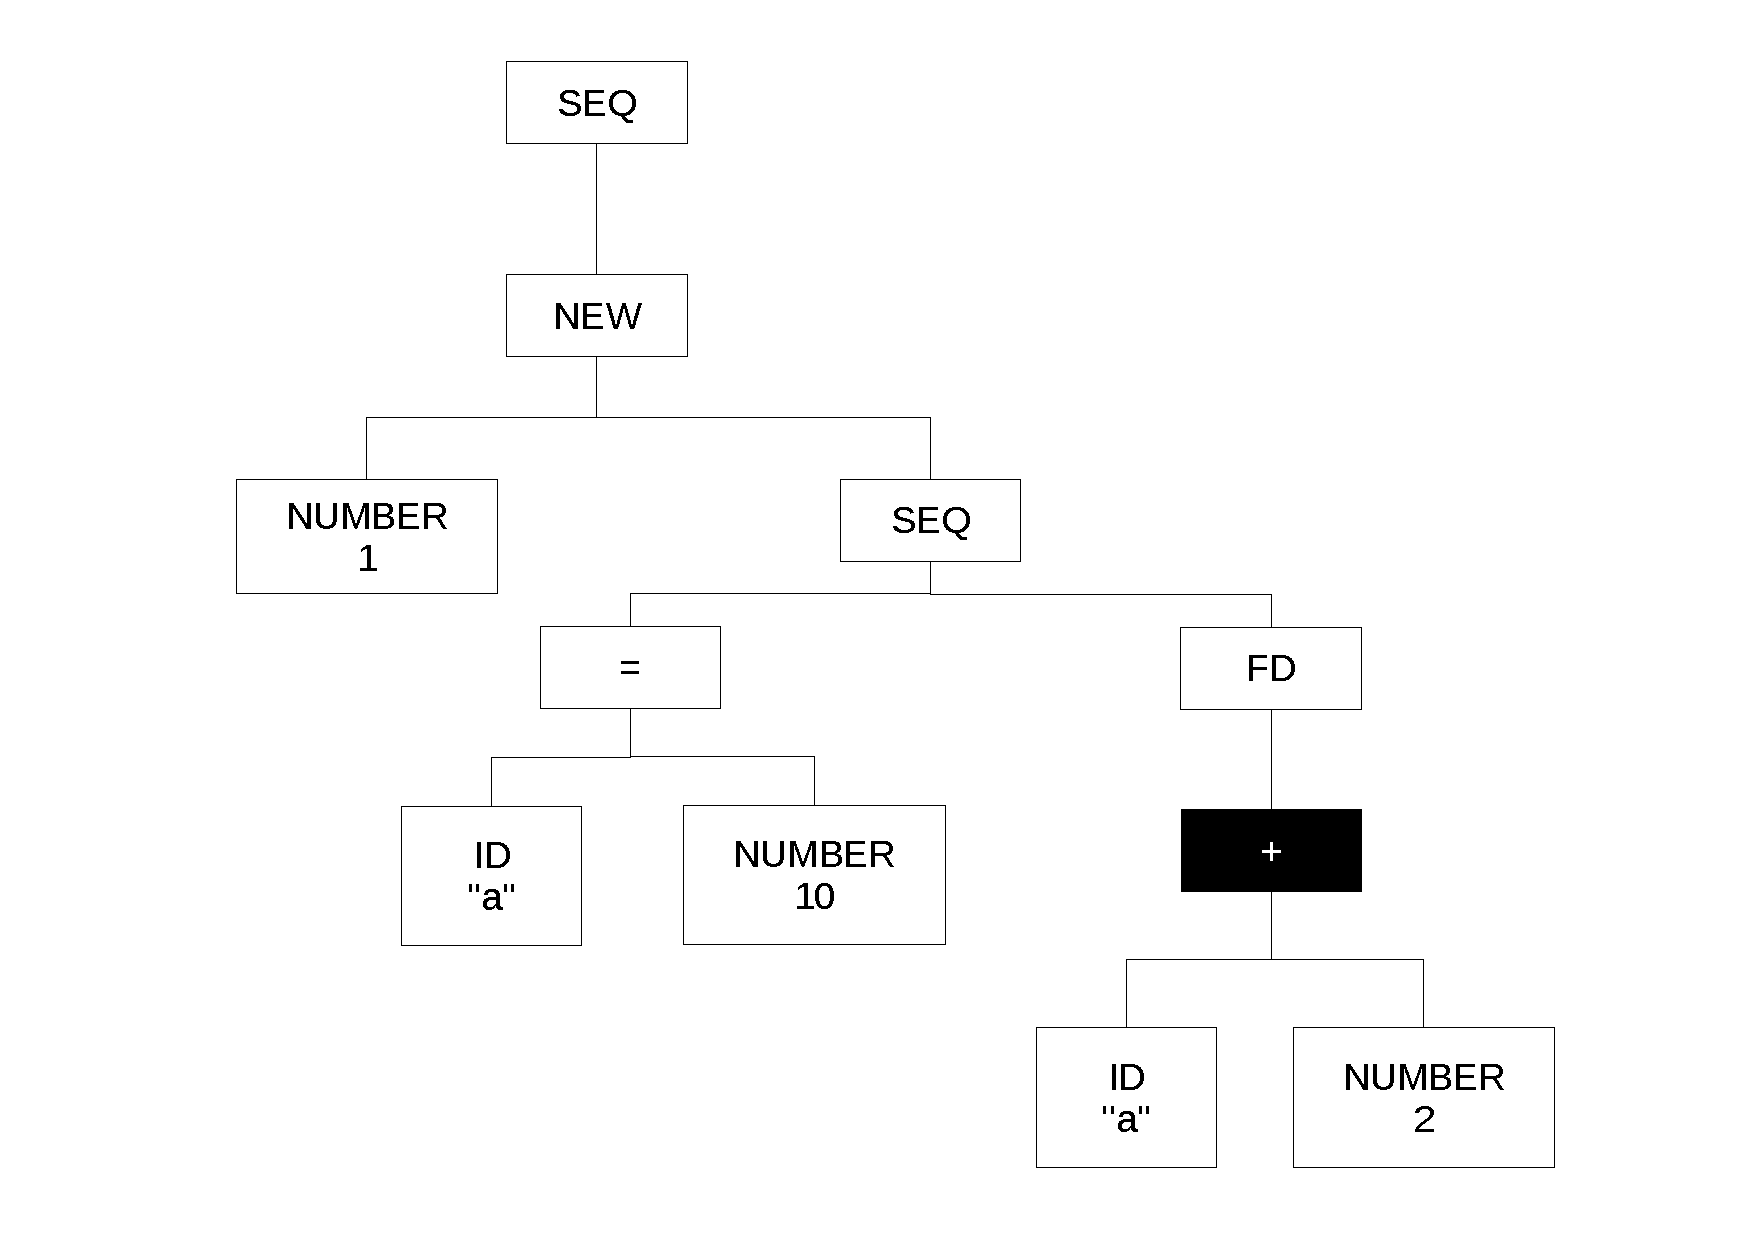
\includegraphics[scale=0.3]{doc/Presentation/img/arbre9.pdf}
\end{frame}

\begin{frame}
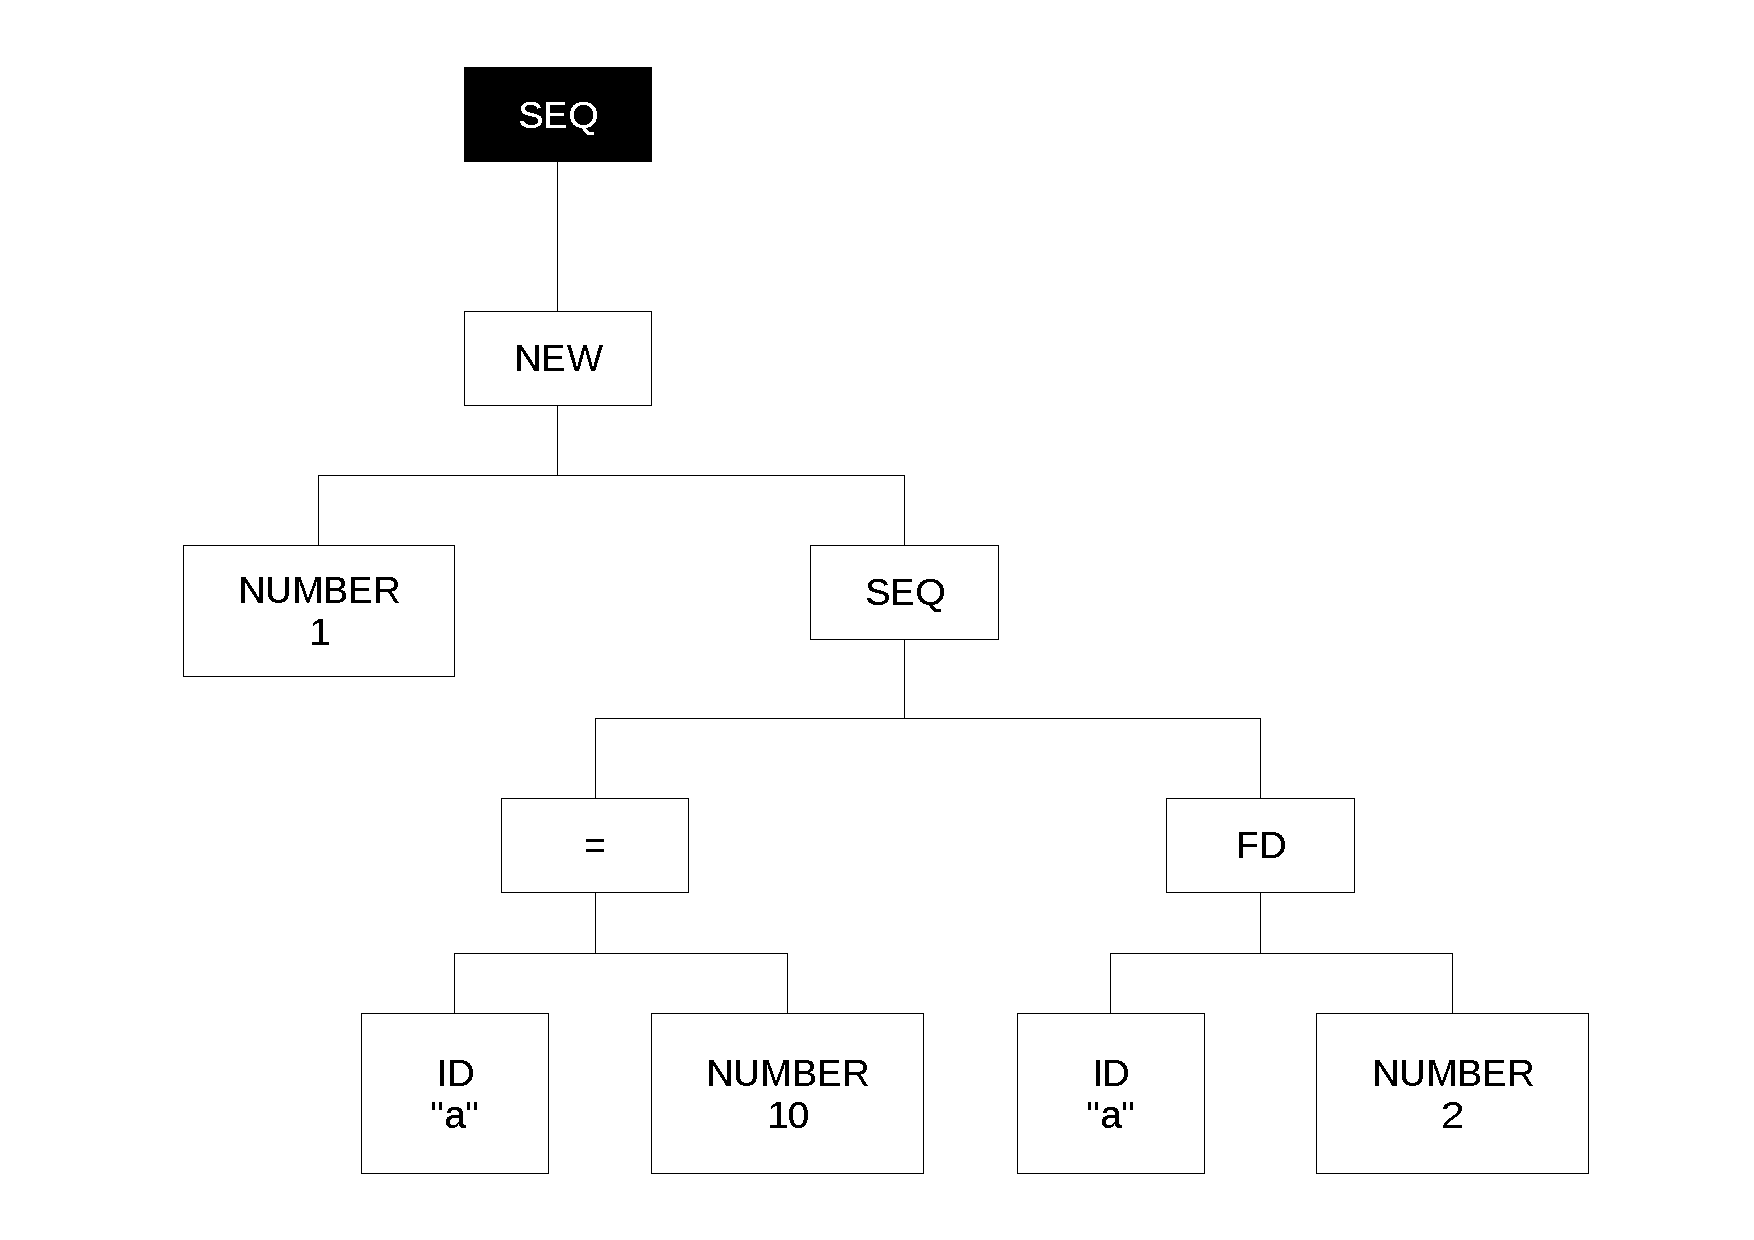
\includegraphics[scale=0.3]{doc/Presentation/img/arbre10.pdf}
\end{frame}

\begin{frame}
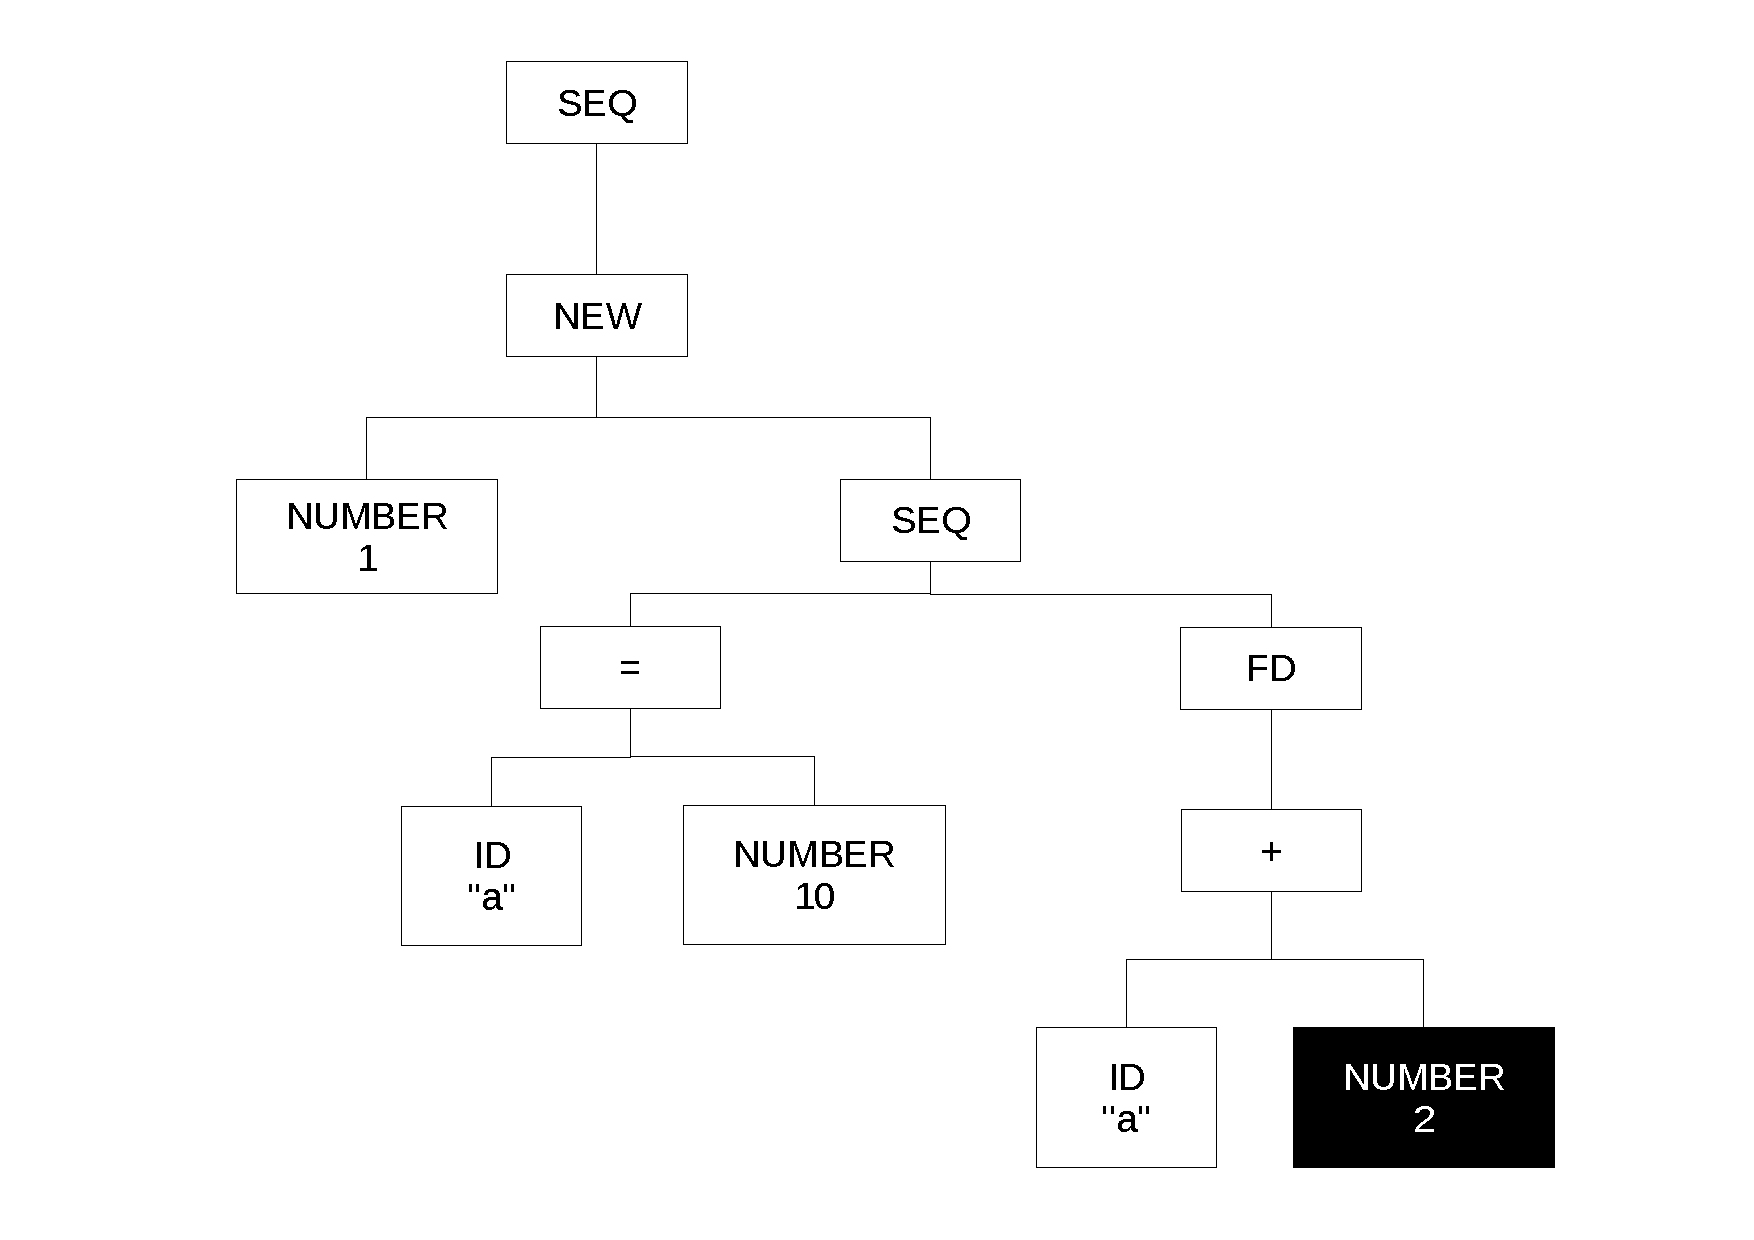
\includegraphics[scale=0.3]{doc/Presentation/img/arbre11.pdf}
\end{frame}

\begin{frame}
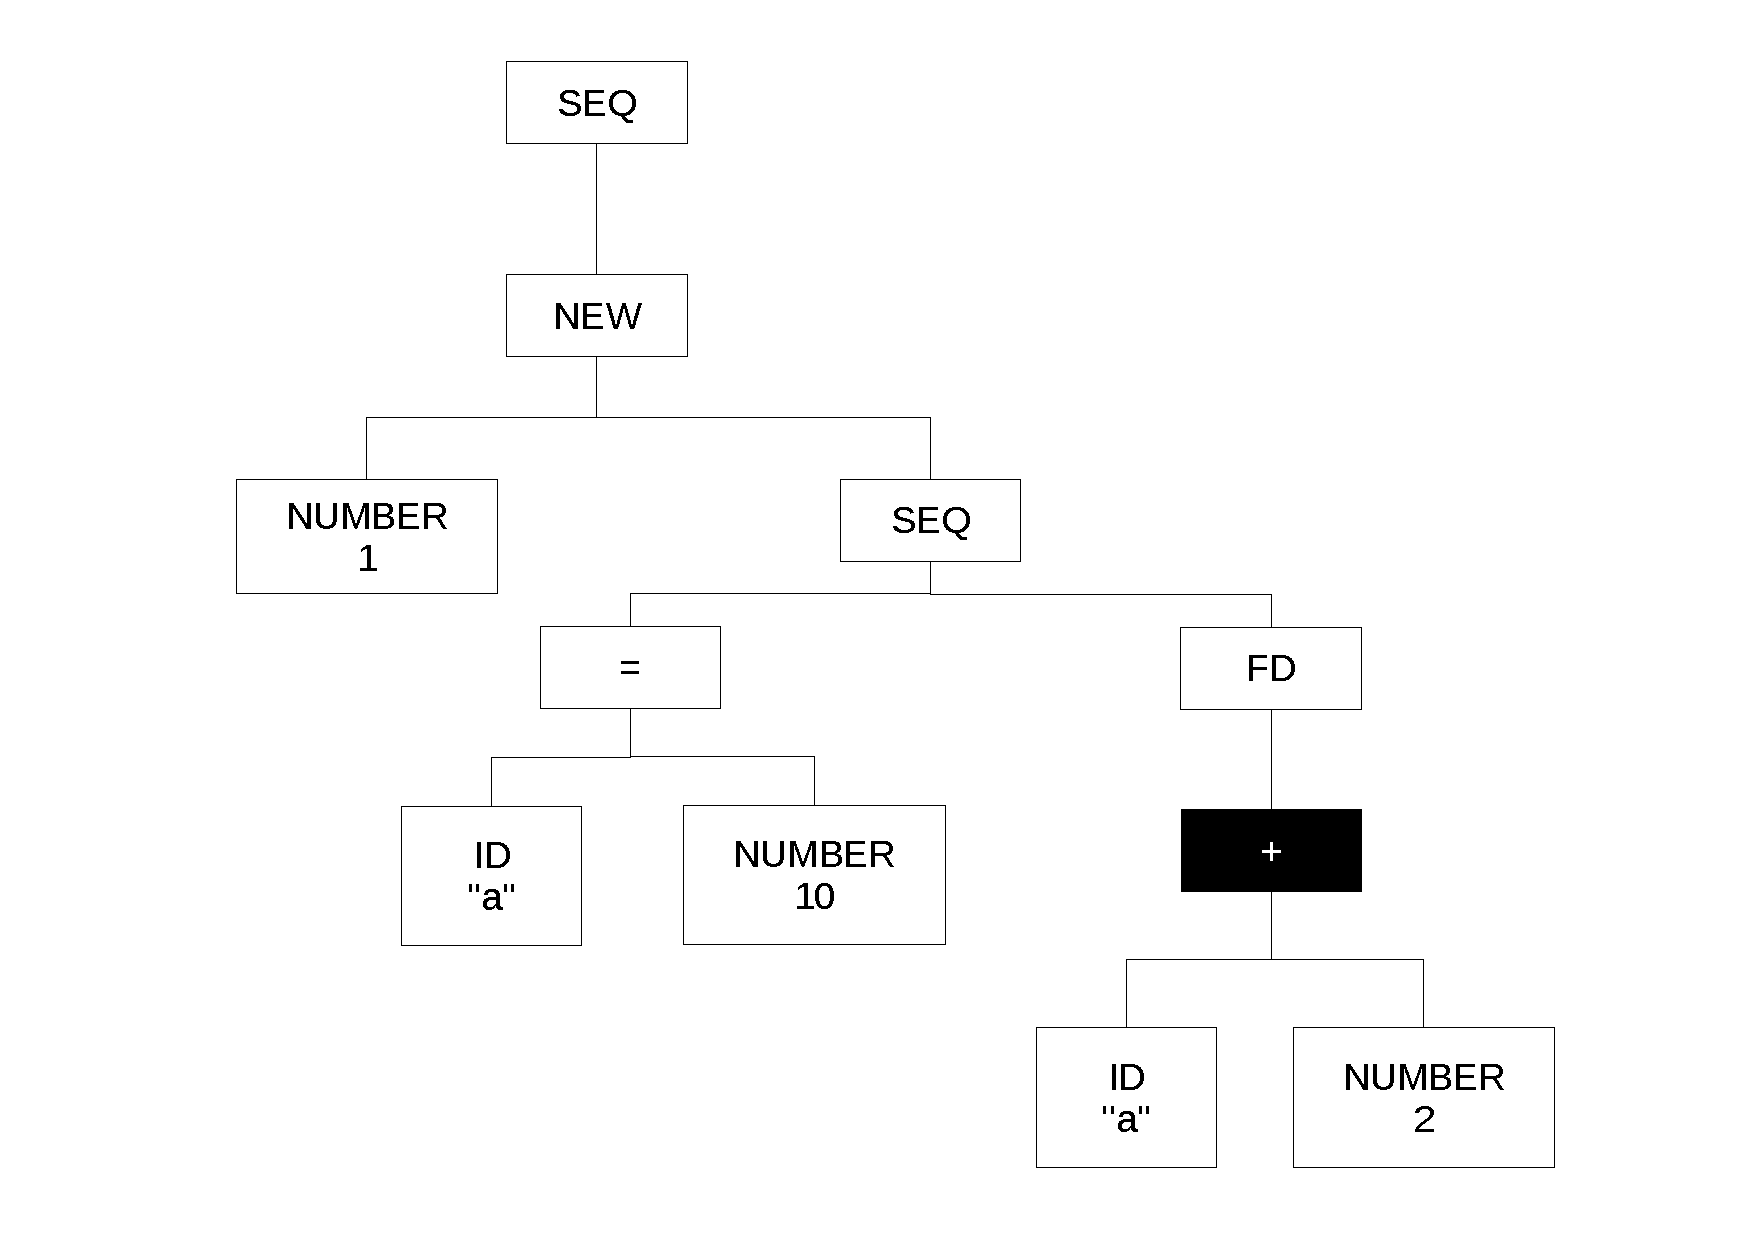
\includegraphics[scale=0.3]{doc/Presentation/img/arbre9.pdf}
\end{frame}

\begin{frame}
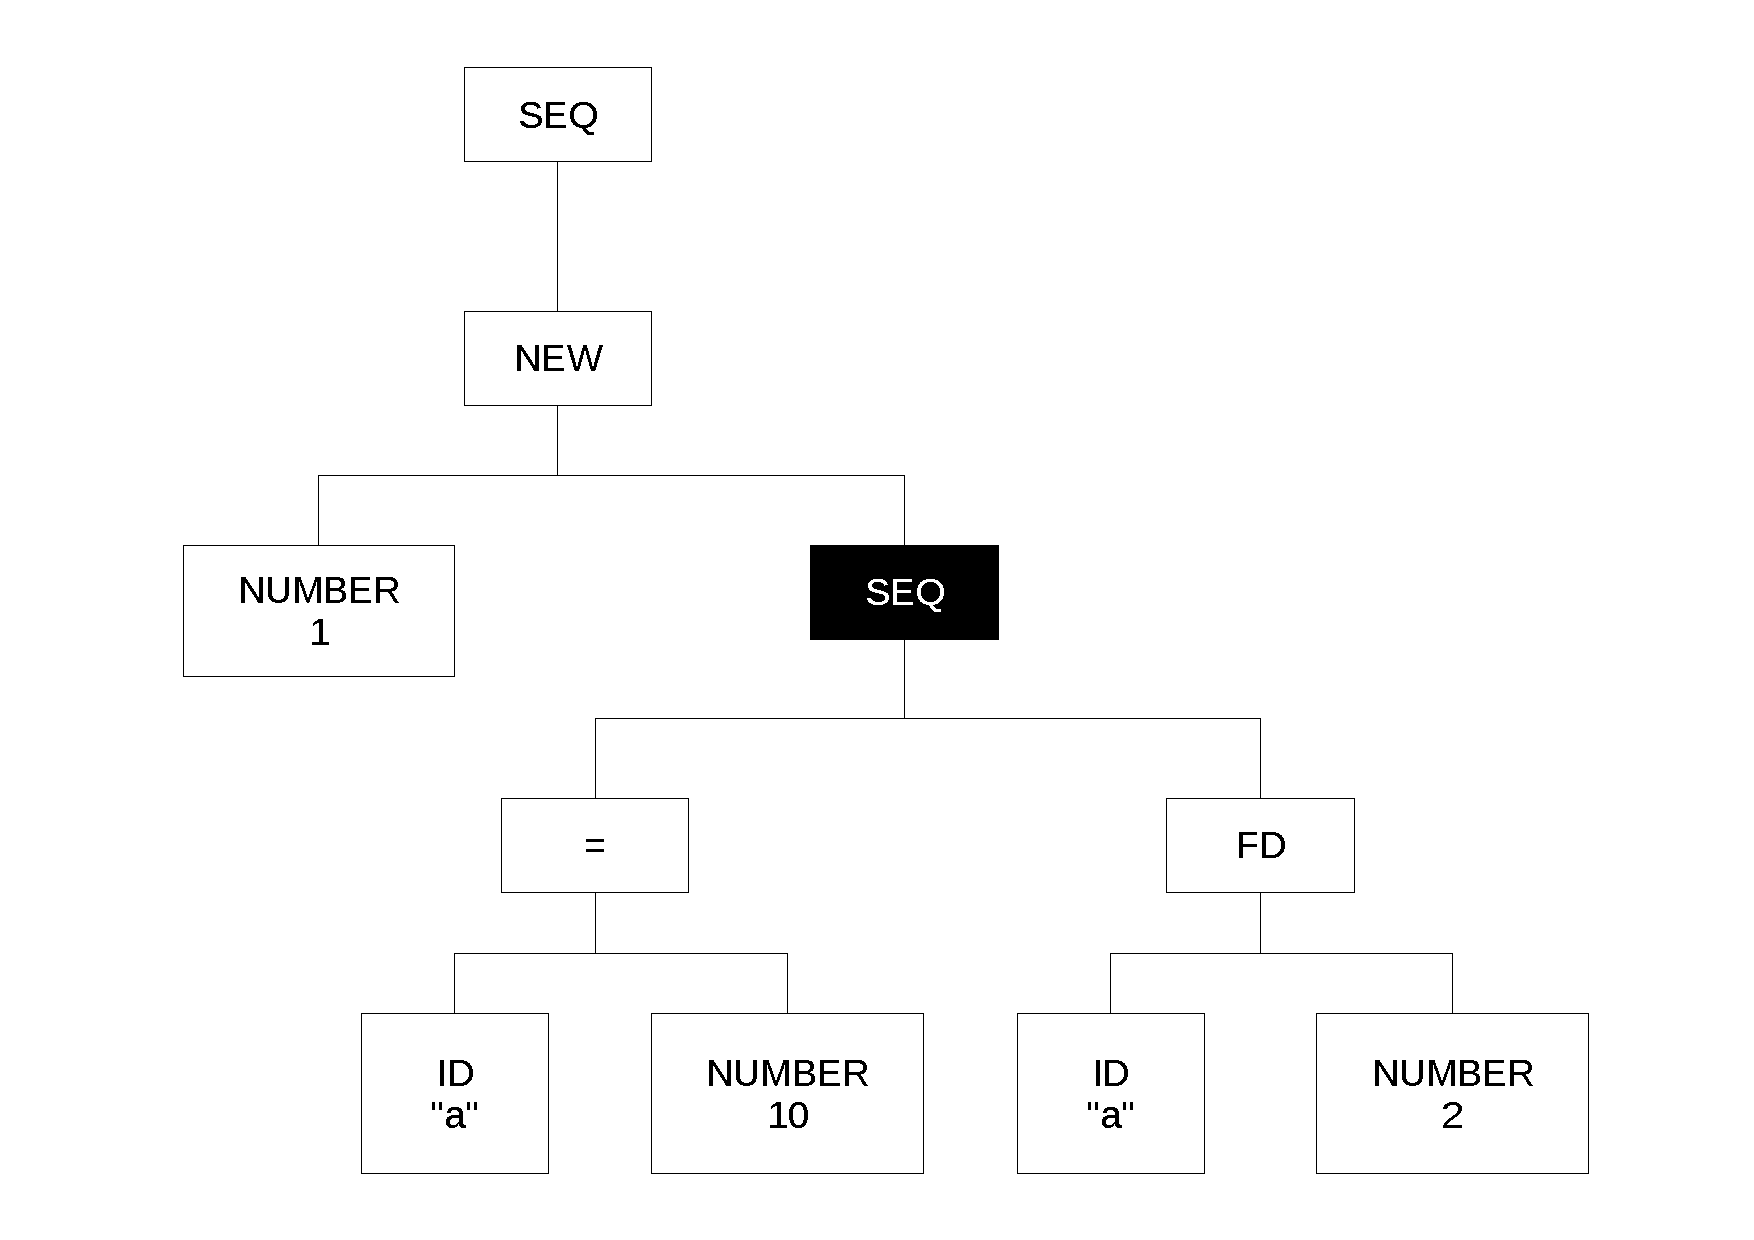
\includegraphics[scale=0.3]{doc/Presentation/img/arbre8.pdf}
\end{frame}

\begin{frame}
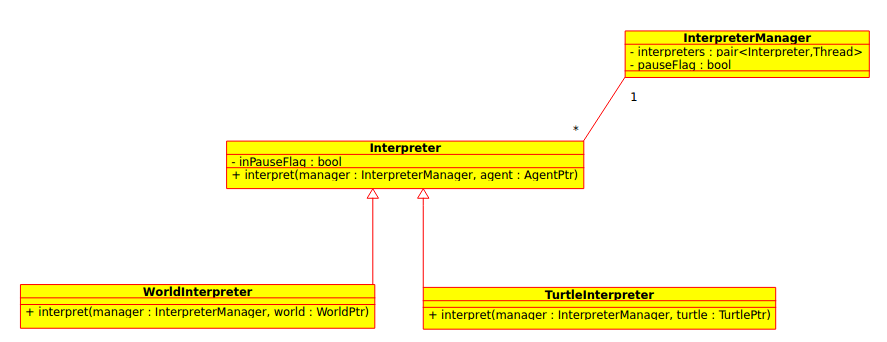
\includegraphics[scale=0.3]{doc/report/uml/interpreterUML.png}
\end{frame}

\begin{frame}[fragile]
Rôles de la classe \verb|InterpretManager|
\begin{itemize}
	\item stocker les couples thread-interprète créés
	\item gérer les interprètes existants
	\item alerter des éventuelles pauses
	\item créer un monde avec les directives choisies
\end{itemize}
\end{frame}

\begin{frame}

L'interprète
\begin{itemize}
	\item analyse un noeud
	\item analyse les enfants du noeud courant
	\item appelle la méthode correspondante du modèle
\end{itemize}
\end{frame}
